%!TEX root = ./main.tex

\begin{table*}[htb]
	%\begin{center}
		\begin{tabular}{rl m{1.9cm} ll}
			\toprule
			Symbol		&	\multicolumn{1}{c}{Meaning} &
				Reference	& Range & units
		\\
		\midrule
			$M_S(0)$
				& Initial number of 
		\\
			$M_1(0)$,
				& susceptible and infected
		\\
		    $M_2(0)$
		    &  mosquitoes.
		\\
		$N_H$
		    & Total Susceptible population
		    &  INEGI (see \cref{sec:Intro})
		    & \num{283493}
		\\
			$b$
			& Biting rate
			&\cite{YasunoM1990}
			&[10.36 , 33.39] & $\si{meals \per week}$ 
		\\
%			$\Lambda_S$
%				& Human birth rate
%				&
%				& 
%					$\mu_H \cdot (N_H - N_{S_{-1}})$
%				& $\si{week^{-1}}$
%		\\
%			$\Lambda_{S_{-1}}$
%				& Human birth rate
%				&
%				& 
%					$\mu_H \cdot N_{S_{-1}}$
%				& $\si{week^{-1}}$
%		\\
			$\Lambda_M$
			& Vector birth rate
			&
			& $\mu_M \cdot N_M$
			& $\si{week^{-1}}$
		\\
			$\mu_M$
			& vector mortality rate
			& \cite{YANG2009}
            & [\num{0.252}, \num{0.763}] 
            & $\si{week^{-1}}$
    \\
			$\mu_H$
			& Human mortality
			&---
			& \num{0.000273973} 
			& $\si{week^{-1}}$
		\\
			$\beta_H$ 
			&	Human infection 
			\\
      & probability  by vectors
			& \cite{Feng1997a} 
			& (\num{0}, \num{0.05}] 
			& ---
		\\
			$\beta_M$
			& Vector infection 
			\\
      & probability by humans
			& \cite{Feng1997a}& (\num{0}, \num{0.05}] & ---
		\\
			$\alpha_{c}$ 
			& Mean recover rate 
			\\
      & from Classic Dengue
			&\cite{Pinho2010}
			& [\num{0.581}, \num{1.75}] & $\si{week^{-1}}$
		\\
			$\alpha_{h}$	& Mean recover rate
			& \cite{Pinho2010} 
			& [\num{0.581}, \num{1.75}] 
			& $\si{week^{-1}}$
		\\
			& from Hemorrhagic Dengue
		\\
			$\sigma$
			& Susceptibility to serotype 
		\\
			& \ac{DENV-2}.
			& \cite{Feng1997a}
			& $(0,5)$
      \\
            $p$ 
            & 
            Ratio of asymptomatic cases
            &
            \cite{balmaseda2006high},
            &
            $[\frac{1}{60}, \frac{1}{30}]$
            & ---
            \\
            & &
            \cite{Chastel2011, Chastel2012a}
            \\
			$\theta$
			& Probability of 
			\\
			& acquire DHF 
			\\
			& as second infection
			\\
			\bottomrule
		\end{tabular}
	%\end{center}
	\caption{Parameter description}
	\label{tbl:parameter_description}
\end{table*}
%!TEX root = ./main.tex

\begin{table*}[htb]
	\begin{center}
		 \begin{tabular}{lll}
			\toprule
			 \multicolumn{3}{c}{
				 \textbf{
					 Parameters (time in  weeks) for
					 \cref{fig:fitting,fig:population_grid}
					 }
				 }
				 \\
			 \midrule
			 $\Lambda_M = \num{30702.6139006}$, &
			 $\Lambda_S = \num{10.2385934233}$, &
			 $\Lambda_{S_{-1}} = \num{1.13762149148}$,
			 \\
			 $\alpha_c = \num{0.686615937276}$, &
			 $\alpha_h = \num{1.41310092256}$, &
			 $b = \num{12.7122333418}$,
			 \\
			 $\beta_H = \num{0.0478488977733}$, &
			 $\beta_H = \num{0.0478488977733}$, &
			 $\beta_M = \num{0.0361065995648}$,
			 \\
			 $\mu_H = \num{0.000273}$, &
			 $\mu_M = \num{0.307170720093}$, &
			 \\
			 $\sigma = \num{1.806480946}$,
			 \\
			 $\theta = \num{0.1887501857}$, &
			 \\
			 $p = \num{0.126295209216}$, &
			 $h = \num{0.000189285714286}$, &
			 \\
			 \\
			 $S(0) = \num{35598.0}$, &
			 $I_{1}(0) = \num{1.0}$, &
			 $I_{2}(0) = \num{1.0}$,
			 \\
			 $M_{S}(0) = \num{120000}$, &
			 $M_{1}(0) = \num{10}$, &
			 $M_{2}(0) = \num{10}$, 
			 \\
			 $S_{-1}(0) = \num{4400.0}$, &
			 $Y_{-1}^{[c]} (0) = \num{0.0}$, &
			 \\
			 $Y_{-1}^{[h]} (0) = \num{0.0}$, &
			 $z(0) = \num{0.252590418433}$, &
			 $Rec(0) = \num{0.0}$, 
			 \\
			 \bottomrule 
		 \end{tabular}
	 \caption{Parameters of numerical example}
	 \end{center}
\end{table*}

\todo[inline]{Discuss above parameters units. Weeks or days}
%
\begin{figure}
	\centering
	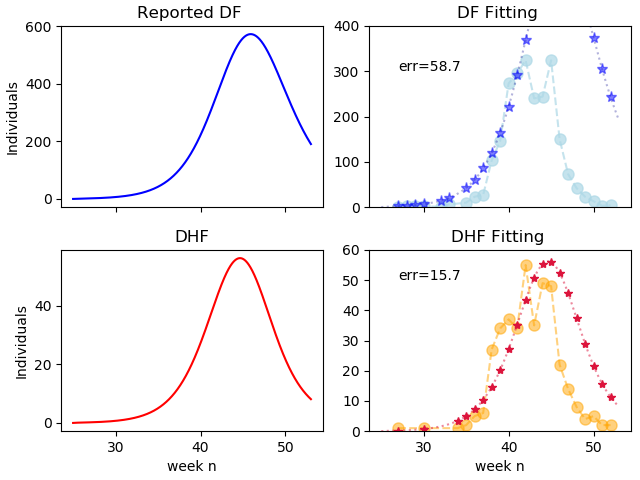
\includegraphics[width=\textwidth, keepaspectratio]{fitting_DF_DHF.png}
	\caption{DF and DHF numerical solutions versus
		Dengue data from 2010 Hermosillo outbreak. Python code and
    data in 
    \href{github}{https://github.com/SaulDiazInfante/Two-strains-dengue-model-data-%
        fitting/tree/master/StochasticSearchPySimplifiedModel}
	}\label{fig:fitting}
\end{figure}

<<<<<<< HEAD
\begin{figure}[htb]
=======
\begin{figure}[h]
>>>>>>> 0f463030b7fe3786d8fc6fc84c6ae076b736d28f
	\centering
	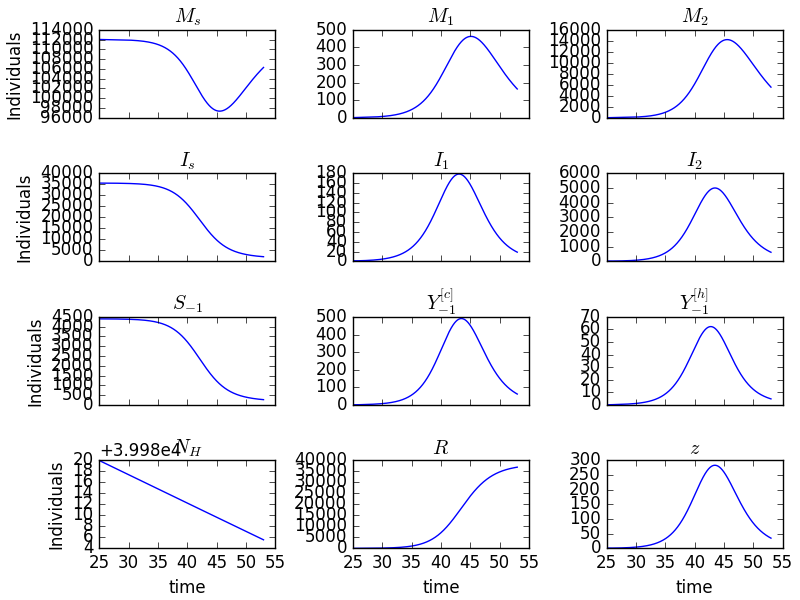
\includegraphics[width=\textwidth, keepaspectratio]{populations_grid.png}
	\caption{Evolutions of each stage.}\label{fig:population_grid}
\end{figure}